\documentclass[19pt,a4pape、、r]{article}
\usepackage{xeCJK}
\usepackage{amsmath}
\setmainfont{STSong}
\usepackage{geometry}
\geometry{left=2.5cm,right=2.5cm,top=2.5cm,bottom=2.5cm}
\setlength{\parindent}{4em}
\usepackage{graphicx}
\usepackage{float}
\title{算法作业8}
\author{孟妍廷2015202009}
\date{2017年11月17日}

\begin{document}
\maketitle
16.2-4证明:使用题目要求中的参数\\
\indent 1.证明最优子结构:\\
\indent 假设$X=x_1,...x_n$是问题的最优解,包含a个补水站,$x_k$是$x_n$的前一个被选择的补水站。
假设$X_1=x_1...x_k$不是是子问题N-m的最优解,它共包含a-1个补水站,而$Y_1=y_i...y_j$是该子问题的最优解,共包含b个补水站
则可知$b<a-1$,故$y_i...y_j,x_n包含的补水站个数为b+1<a-1+1=a$,则$y_i...y_j,x_n$比$X=x_1,...x_n$更优,产生矛盾。\\
\\
\indent 2.证明贪心选择性质\\
\indent 设 $X = x_1 , ..., x_n$是贪心算法求得的解, 设问题的最优解为 $Y = y_1 ....y_n$ 则存在k使得$y_k\ne x_k$ 为最小下标,否则Y=X得证。\\
\indent 首先, 由于 $x_k$ 是距离 $x_{k−1}$ 最远的在 m 范围内的补水站,则可以证明 $y_k < x_k$,则 $y_n −y_k > x_n −x_k$ 剩余的距离变长,需要选择的补水站的个数只可能增加,不符合最优解,因此只能$x_k=y_k,对于任意k$。\\
\indent 因此得证 Y=X\\
\\
\indent 16-2\\
\indent a.由于是非抢占的,所以每次都选择剩余的任务中运行时间最短的任务,算法如下:\\
\indent $solution(p)\\
\indent\quad let\ c[1...n]\ be\ a\ new\ array\\
\indent\quad sort(p)\ \ //使得\ p_1\le p_2\le p_3\cdot\cdot\cdot\\
\indent\quad c_1\ =\ p_1\\
\indent\quad for\ i=2\ to\ n\\
\indent\quad\quad c_i\ = \ c_{i-1}+p_i\\
\indent\quad avg=0\\
\indent\quad for\ i=1\ to\ n\\
\indent\quad\quad avg=avg+c_i\\
\indent\quad avg=\frac{avg}{n}\\
\indent\quad return\ avg$\\
\indent 时间复杂度为O(nlgn).\\
\indent 证明最优性:\\
\indent 1.最优子结构\\
\indent 假设$X=x_1....x_n$是最优解,而$X_1=x_1....x_{n-1}$不是除第$x_n$任务的n-1个任务的最优解,而$Y_1=y_i...y_{n-1}$是该子问题的最优解
可知$\sum_{i=x_1}^{x_{n-1}}c_i>\sum_{i=y_1}^{y_{n-1}}c_i$,则$\sum_{i=x_1}^{x_{n-1}}c_i+c_{x_n}>\sum_{i=y_1}^{y_{n-1}}c_i+c_{x_n}$
与$X=x_1....x_n$是最优解矛盾,故最优子结构得证\\
\indent 2.贪心选择性质\\
\indent 设$X=x_1....x_n$是贪心算法选择任务的下标顺序,设该问题的最优选择下标顺序为$Y = y_1 ....y_n$ 则存在k使得$y_k\ne x_k$ 为最小下标,否则Y=X得证。\\
\indent 由于贪心算法选择的是运行时间最短的任务,则可知$p_{x_k}<p_{y_k}$。记任务$a_{x_k}$在最优解中出现的位置为i(i>k),若将最优解中任务$a_{y_k}$与任务$a_{x_k}$调换一下顺序,则第k+1到i-1个任务的结束时间都缩短了$p_{y_k}-p_{x_k}$,而第i个到第n个任务的结束时间没有变化,总体的平均运行时间缩短,说明Y不是最优解,故贪心选择性质得证。\\
\indent b.由于任务是可以抢占的,所以策略是记录每个任务的剩余时间,在当前可以开始的任务中选择
剩余时间最短的任务执行,当下一组任务到来时,比较该组任务剩余时间最短的任务与当前任务,若小于当前任务的剩余时间就抢占。\\
\indent 算法如下:\\
\indent $solution(p,r)\\
\indent\quad let\ c[1...n]\ be\ a\ new\ array\\
\indent\quad sort(r,p)\ \ //使得\ r_1\le r_2\le r_3\cdot\cdot\cdot,同时在排序时同步交换p_i,使得p_i和r_i对应同一a_i\\
\indent\quad cur=\infty\ \ //记录当前被执行的任务\\
\indent\quad for\ i=1\ to\ n\\
\indent\quad\quad for\ j=1\ to\ n\\
\indent\quad\quad\quad if\ r_j\ge r_i\ and\ p_j<cur\\
\indent\quad\quad\quad\quad cur=j\ \ //找出剩余时间最短的任务作为新任务\\
\indent\quad\quad if\ p_j\ge r_i\\
\indent\quad\quad\quad p_j=p_j-r_i\\
\indent\quad\quad\quad c_j=c_j+r_i\\
\indent\quad\quad else\\
\indent\quad\quad\quad p_j=0\\
\indent\quad\quad\quad c_j=c_j+p_j\\
\indent\quad avg=0\\
\indent\quad for\ i=1\ to\ n\\
\indent\quad\quad avg=avg+c_i\\
\indent\quad avg=\frac{avg}{n}\\
\indent\quad return\ avg$\\
\indent 时间复杂度为$O(n^2)$.\\
\indent 证明最优性:\\
\indent 1.最优子结构\\
\indent 假设$X=x_1....x_m(m>n)$是最优解,而$X_1=x_1....x_{m-1}$不是除最后一次选择之外的前m-1次选择的最优解,而$Y_1=y_i...y_{m-1}$是该
子问题的最优解。\\
在该子问题执行完毕之后,所有的任务应该都可以开始或者已经执行完毕,所以问题相当于问题a,故证明过程同上。\\
\indent 2.贪心选择性质\\
\indent 设$X=x_1....x_m$是贪心算法选择任务的下标顺序,设该问题的最优选择下标顺序为$Y = y_1 ....y_m$ 则存在k使得$y_k\ne x_k$ 为最小下标,否则Y=X得证。\\
\indent 由于贪心算法选择的是当前可以执行的剩余时间时间最短的任务,则可知$p_{x_k}<p_{y_k}$。故若在该阶段将选择这行的任务替换为任务$a_{x_k}$,则之后的阶段被选择的任务的结束时间都将提前,总体的平均运行时间缩短,说明Y不是最优解,故贪心选择性质得证。\\
\\
\indent 16.2-3\\
\indent 假设有n个字符,第1个字符有n-1个1,其余字符有n-i个1加末尾一个0.\\
\indent 如图所示\\
\begin{figure}[H]
 \centering
 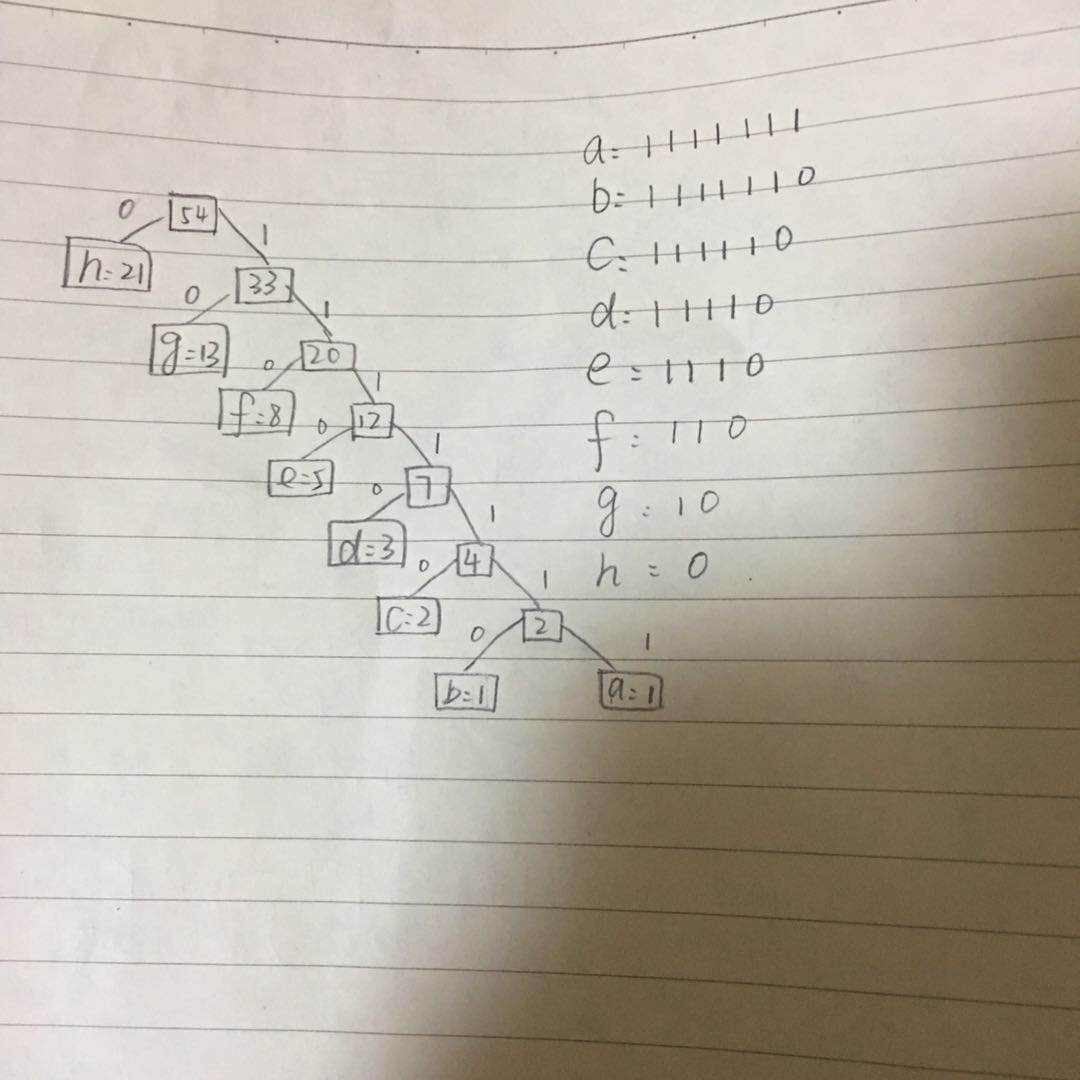
\includegraphics[scale=0.3]{8.jpeg}
\end{figure}






\end{document}